%%%%%%%%%%%%%%%%%%don't forget if needed %%%%%%%%%%%%%%%%%%%%%
%\section[toc version]{title version%
%              \sectionmark{head version}}
%\sectionmark{head version}
%%%%%%%%%%%%%%%%%%%%%%%%%%%%%%%%%%%%%%%%%%%%%%%%%%%%%%%%%%%%%%
\def\titcourt{Numerical simulation of 3D convection and PCM}
\def\titlong{Numerical simulation of 3D convection and PCM configurations using domain decomposition method}
%%%%%%%%%%%%%%%%%%%%%%%%%%%%%%%%%%%%%%%%%%%%%%%%%%%%%%%%%%%%%%%%
\chapter[\titlong]{\titlong%
              \chaptermark{\titcourt}}
\chaptermark{\titcourt}
\label{chap-3D-SIMULATION}
%%%%%%%%%%%%%%%%%%%%%%%%%%%%%%%%%%%%%%%%%%%%%%%%%%%%%%%%%%%%%%%%
%%%%%%%%%%%%%%%%%%%%%%%%%%%%%%%%%%%%%%%%%%%%%%%%%%%%%%%%%%%%%%%%
Several sections of this chapter are from the paper [G. Sadaka, A. Rakotondrandisa, F. Luddens, C. Lothod�, P-H. Tournier, I. Danaila, \textit{Parallel finite-element codes for the simulation of solid-liquid phase-change systems with natural convection}, to be submitted, 2019].

We present in this chapter parallel computations of three-dimensional liquid-solid phase-change systems involving natural convection.
We use the recent library \texttt{ffddm} that makes available in FreeFem++ a state-of-the-art scalable Schwarz domain decomposition method (DDM).
Our motivation to expand our numerical model to 3D configurations is drawn by the lack of publications in the literature presenting accurate 3D simulations of phase-change materials.
Also, experimental investigations against which we have validated our numerical method in previous chapters involve three-dimensional effects that we have assumed to be negligible in our comparisons.
The latter assumption is however not valid for high $\Ray$ numbers.

The main feature of our numerical approach is the use of 3D adaptive mesh, performed using \textit{mmg3d} library.
\textit{Mmg3d} is a 3D software developed by \cite{dobrzynski:hal-00681813}, which allows to remesh an initial mesh made of tetrahedra.
The metrics for the mesh adaptation are computed using \textit{mshmet} library, which provides anisotropic metrics based on solution variations.
Since the mesh adaptivity procedure is based on a sequential algorithm, we compute first the metrics with respect to the coarse mesh. 
Then, finer local meshes are generated in parallel during the mesh decomposition step in order to reach the desired level of refinement for the subdomains.
We use \textit{Metis} library to split the domain into subdomains.
The number of layers of mesh elements in the overlap region between subdomains is set to $2$ for all subsequent simulations.
For three-dimensional applications, direct solvers used in the framework of 2D problems are not appropriate and iterative methods must be employed since memory requirements for the \textit{LU} decomposition would rapidly exceed the capacity of available computers.
The linear system of equations resulting from the Newton linearization are thus solved using parallel \textit{GMRES} Krylov method.
Since it is well known that iterative methods can suffer from convergence problems, we adapt the number of subdomain in such a way that each processor could handle $1,000$ tetrahedra.
The Optimized Restricted Additive Schwarz (ORAS) preconditioned \textit{GMRES} solver proved to be extremely efficient since around 30 iterations were necessary to get a residual of $10^{-9}$ for each Newton iteration.
%We note that in all numerical simulations, a quadratic ($\PP_2$) discretization of $\theta$ was used.

The remainder of this chapter is as follows.
In Sec. \ref{sec: natconv-air-3D}, we first validate the 3D convection of air in a cubic cavity against numerical benchmark by \cite{Wakashima-2004},
and compare together the solutions obtained using the parallel and the sequential algorithms.
Second, the convection of water is investigated in Sec. \ref{sec-3D-water-convec}. %to illustrates the capability of our method to deal with non-linear body force $f_B$ and to capture accurately interfaces, mainly the density inversion.
Then, the melting of n-octadecane PCM inside 3D enclosure is addressed in Sec. \ref{sec-3D_melting}.
We finally present in Sec. \ref{sec-3D_Water_FREEZING} the challenging numerical simulation of water freezing.

\section{Numerical simulation of the natural convection of air in a cubic cavity}\label{sec: natconv-air-3D}
 Following the same argument of increasing gradually the complexity of computed cases, that was outlined in Chapters \ref{chap-NATCONV} and \ref{chap-MELTING}, we start by presenting the natural convection of air. 
 This case involves a linear buoyancy force $f_B$, and include gradually additional non-linearities.
The physical parameters are the same that used in the 2D simulations ($\Prd = 0.71$) and we investigate Rayleigh numbers ranging from $\Ray=10^4$ to $\Ray=10^6$. 
The walls are rigid and impermeable. The vertical walls at $x=0$ and $x=1$ are isothermal and have different temperatures $\theta_h = 0$ and $\theta_c = 1$, respectively. The remaining walls are considered adiabatic. 
The fluid is initially at rest and the temperature is linearly distributed from the cold to the hot walls.
We solve the steady Eq. \eqref{eq-weak-steady} by increasing smoothly the parameter $\alpha$ before the Boussinesq term (which can be assimilated to a Rayleigh continuation step) with a maximum of $6$ steps for $\Ray = 10^6$.

\begin{figure}
\begin{minipage}{\linewidth}
\begin{center}
 {\includegraphics[width=.95\textwidth]{\figpath/Fig_cap_natconv/Validation_3D_seq_T1}}
\end{center}
\end{minipage}
\caption{Natural convection of air in a differentially heated cavity using $3-$D configurations. Temperature contours at the mid-plane of ($y=0.5$); comparison with the results of \cite{Wakashima-2004} (left images). }
\label{fig-3DT} 
\end{figure}
We first compare the current simulation with the numerical data of \cite{Wakashima-2004}. 
These authors used a forth order finite difference method, with a vorticity-stream function formulation with different uniform meshes of  $120 \times 120 \times 120$ grid nodes.
Our results were obtained using uniform grids of $ 40 \times 40 \times 40$.
Since the converged flow pattern and temperature distributions are symmetrical with respect to the center of the cavity for the investigated Rayleigh number,
we display in 
Fig. \ref{fig-3DT} the temperature field at the mid section ($y = 0.5$), for each of the three Rayleigh numbers $\Ray = 10^4$ (top), $\Ray = 10^5$ (middle), $\Ray = 10^6$(bottom).  
On the left we display the numerical results of \cite{Wakashima-2004} and on the right the present simulation.
The comparison with the benchmark solution exhibits qualitatively a good agreement. %with the considered test case.
The higher the Rayleigh number, the finer the thermal boundary layer thickness is in the vicinity of the vertical walls.
One can also notice the stagnant fluid with stratified temperature in the center of the domain in both numerical solutions.

A more accurate comparison is addressed in Tab. \ref{tab-3D-locU} between the present simulation and numerical data from the literature.
\begin{table}[!h]
   \begin{center}
      \begin{tabular}{*{3}{cl}}
           & $u_{max}$ ($y_{max}$) & $v_{max}$ ($x_{max}$) \\ \toprule
           $\Ray = 10^4$ & $0.198094$ ($0.826772$) & $0.220973$ ($0.11811$) \\ 
           \cite{Wakashima-2004} & $0.1984$ ($0.8250$) & $0.2216$ ($0.1177$) \\
           \cite{Raluca2013} & $0.1859$ ($0.8230$) & $0.2234$ ($0.1172$) \\ \hline
           
           $\Ray = 10^5$ & $0.140367$ ($0.850394$) & $0.245454$ ($0.0629921$) \\ 
           \cite{Wakashima-2004} & $0.1416$ ($0.8500$) & $0.2464$ ($0.0677$) \\
           \cite{Raluca2013} & $0.1461$ ($0.8540$) & $0.2459$ ($0.0703$) \\ \hline
           
           $\Ray = 10^6$ & $0.0809247$ ($0.858268$) & $0.257719$ ($0.0393701$) \\ 
           \cite{Wakashima-2004} & $0.08111$ ($0.8603$) & $0.2583$ ($0.0323$) \\ 
           \cite{Raluca2013} & $0.0830$ ($0.8550$) & $0.2553$ ($0.03905$) \\ \bottomrule       
           
               \end{tabular}
   \end{center}
   \caption{Natural convection of air in a $3-$D differentially heated cavity. Maximum values $u_{max}$ and $w_{max}$ of the velocity profiles at mid-domain ($x = 0.5$ and $z=0.5$, respectively) and their locations $z_{max}$ and $x_{max}$. Comparison with benchmark solutions of \cite{Wakashima-2004} and numerical data of \cite{Raluca2013} for $\Ray = 10^4$, $\Ray = 10^5$, $\Ray = 10^6$.}
   \label{tab-3D-locU}
\end{table}

\noindent We assess the maximum velocity values and their corresponding location with benchmark solution of \cite{Wakashima-2004} and numerical results of \cite{Raluca2013}.
Our results show a good convergence on a mesh $3$ times coarser than the one proposed by  \cite{Wakashima-2004}.
A good agreement is found for all values of the Rayleigh number.
For $\Ray = 10^4$ the current simulation shows a relative difference of $0.15 \%$ for $u_{max}$ and $0.28 \%$ for $v_{max}$. %with the latter.
Larger differences of $6.55 \%$ is found with the results reported by \cite{Raluca2013}. 
We recall that \cite{Raluca2013} used a second-order finite difference scheme on a $64 \times 64 \times 64$ grid.
For $\Ray = 10^5$ and $10^6$ the results are in good agreement with both references.


Further comparison of the parallel solver with the sequential algorithm is offered in Tab. \ref{tab-T1} for all cases. 
We compute $L^2$ and $L^\infty$ norms of the velocity and the temperature.
The number of subdomains varies from $28$ to $70$ for $1.8$ millions of unknowns. %to assess the consistency of our method with the number of subdomains.
The difference between both algorithms is of order of $10^{-6}$
and we do not observe a large variation of the error when the number of subdomains is increased.
The comparison with the sequential algorithm was limited to the $40 \times 40 \times 40$ grid, since the simulations are highly demanding in CPU time.
For the highest value of the Rayleigh number, the steady state computation required $57$ CPU hours and $3$ runs (restarts) with $120$ Go of memory for the sequential algorithm, . 
The computational time is considerably reduced using DDM and 3D simulations. This becomes affordable  since only $21$ CPU minutes were necessary with $70$ processors to compute the same case with an error of $6.02152 \cdot 10^{-6}$ on $\vec u$ and $ 4.50094 \cdot 10^{-6} $ on $\theta$.\\

\begin{table}[!h]
	\begin{center}
		\begin{tabular}{|*{6}{c|}}
			\hline
			 $\Ray$ & \em{nb proc }                  & $||u||_{2}$                        & $||u||_{\infty}$                & $||T||_{2}$              & $||T||_{\infty}$\\ \hline \hline
			\multirow{4}{*}{$10^4$} & 28 & $1.12496 \cdot 10^{-6}$ & $3.1 \cdot 10^{-6}$ & $ 3.09966 \cdot 10^{-6} $ & $7 \cdot 10^{-6}$ \\% \hline
			\cline{2-6}
			& 42 & $1.53698 \cdot 10^{-6}$ & $5.1 \cdot 10^{-6}$ & $ 3.23352 \cdot 10^{-6} $ & $8 \cdot 10^{-6}$ \\ \cline{2-6} %\hline 
			& 56 & $1.55576 \cdot 10^{-6}$ & $5.1 \cdot 10^{-6}$ & $ 3.4342 \cdot 10^{-6} $ & $8 \cdot 10^{-6}$  \\ \cline{2-6} %\hline
			& 70 & $1.25622 \cdot 10^{-6}$ & $3.6 \cdot 10^{-6}$ & $ 3.56048 \cdot 10^{-6} $ & $8 \cdot 10^{-6}$ \\ \hline \hline
			\multirow{4}{*}{$10^5$} & 28 & $1.73254 \cdot 10^{-6}$ & $6.1 \cdot 10^{-6}$ & $ 2.40467 \cdot 10^{-6} $ & $7 \cdot 10^{-6}$ \\% \hline
			\cline{2-6}
			& 42 & $2.84973 \cdot 10^{-6}$ & $7.78 \cdot 10^{-6}$ & $ 3.53003 \cdot 10^{-6} $ & $9 \cdot 10^{-6}$ \\ \cline{2-6} %\hline 
			& 56 & $3.00832 \cdot 10^{-6}$ & $7.39 \cdot 10^{-6}$ & $ 4.17769 \cdot 10^{-6} $ & $1.1 \cdot 10^{-5}$  \\ \cline{2-6} %\hline
			& 70 & $3.68118 \cdot 10^{-6}$ & $9 \cdot 10^{-6}$ & $ 4.70846 \cdot 10^{-6} $ & $1.2 \cdot 10^{-5}$ \\ \hline \hline
			\multirow{4}{*}{$10^6$} & 28 & $6.61804 \cdot 10^{-6}$ & $1.826 \cdot 10^{-5}$ & $ 3.46504\cdot 10^{-6} $ & $1.1 \cdot 10^{-5}$ \\% \hline
			\cline{2-6}
			& 42 & $5.93966 \cdot 10^{-6}$ & $1.5 \cdot 10^{-5}$ & $ 3.98082 \cdot 10^{-6} $ & $1.2 \cdot 10^{-5}$ \\ \cline{2-6} %\hline 
			& 56 & $7.05144 \cdot 10^{-6}$ & $1.9247 \cdot 10^{-5}$ & $ 5.0044 \cdot 10^{-6} $ & $2 \cdot 10^{-5}$  \\ \cline{2-6} %\hline
			& 70 & $6.02152 \cdot 10^{-6}$ & $1.68 \cdot 10^{-5}$ & $ 4.50094 \cdot 10^{-6} $ & $1.8 \cdot 10^{-5}$ \\ \hline
		\end{tabular}
	\end{center}
	\caption {Natural convection of air in a $3-$D  differentially heated cavity. Comparison between sequential and DDM algorithm for uniform grids of $40 \times 40 \times 40$ points. }
	\label{tab-T1}
\end{table}

\newpage
\section{Numerical simulation of the natural convection of water in a cubic cavity} \label{sec-3D-water-convec}

In this section, we simulate the natural convection of water inside cubic cavity using adaptive $3$D meshes.
The dimensionless parameters are the same that used in Chapter \ref{sec: natconv-water} ($\Ray=2.518084\cdot 10^{6}$ and $\Prd=6.99$).
We impose cold dimensionless temperature $\theta_c = 0$ at $x=1$ (right wall), hot temperature $\theta_h = 1$ at $x=0$ (left wall), and a homogeneous Neumann boundary condition at the remaining walls.
Dirichlet boundary condition $\vec u = 0$ is prescribed over the whole boundary $\partial \Omega$.
In view of anomalous thermal variation of water density, we adapt the mesh along $\theta = 0.4$ to capture correctly the flow structure.
The main limitation of 3D simulations of water convection in the literature is the size of the mesh resolution when fixed grid models are used.
As an example, \cite{Giangi-2000} and \cite{Kowalewski-2003}  presented a mesh sensitivity analysis, and concluded that even by using $81^3$ grid points, the variation of the velocity was still significant,
making the problem computationally expensive. %, limiting their analysis.
%Hence, using adaptive mesh helps considerably to combine accuracy and efficiency.

The temperature distribution and the corresponding adapted mesh for the steady state computation is shown in Fig. \ref{fig-3D_Water_convec}a. 
The blue region denotes the cold water trapped by the abnormal fluid recirculation and the red region the hot fluid driven by the upper clockwise circulation.
A zoom of the mesh at the mid-plane is also offered in Fig. \ref{fig-3D_Water_convec}b.
Smaller tetrahedra are clearly observed in the vicinity of the walls, where a spiral movement of the fluid occurs along the walls, and between the two counter-rotating circulation patterns.
A minimum edge length $h_{min} = 3.33 \cdot 10^{-3}$ is used along the maximum density variation, and $h_{max} = 0.15$ in the stagnant fluid region.
The combined mesh adaptation strategy and the efficient parallel algorithm, allows to reduce considerably the computational time. 
Only $5012.04$ CPU seconds were necessary to compute the steady solution with $500,000$ tetrahedra using $56$ processors, while \cite{michalek2005natural} needed $3.6  \times 10^5$ CPU seconds to compute the steady solution with a $81^3$ fixed grid.

In many cases, it is convenient to perform two-dimensional numerical simulations, to reduce the computational effort and allow many simulations to be achieved in a realistic time.
However, Fig. \ref{fig-3D_Water_convec}b shows that the three-dimensionality of the flow in cube shape cavity affects the topology of the iso-surface $\theta=0.4$.
\cite{Giangi-2000} assessed on the effect of three-dimensionality in both convection and freezing of water and they noted that only the flow in the symmetry plane can be considered as two-dimensional.
The no-slip velocity and the adiabatic thermal boundary conditions at the side walls enhance the three-dimensional effect near the walls.
Furthermore, these authors noted that, even though the temperature profiles at the central cross-section of the cavity match well for both $2$ and $3$D solutions in their numerical simulations, important differences between two and three-dimensional velocity profiles are present. %at some points.

In Figs. \ref{fig-3D_Water_convec}d-f, we plot the velocity profiles along the vertical line passing through the velocity saddle point, where normal and abnormal convection streams collide in the vicinity of the cold wall.
For the $\vec e_z$ component of the velocity profile, along $z-$ direction at $x = 0.93$, we could compare both two and three-dimensional simulations with available $3$D simulation of \cite{Kowalewski-2003}.
Triangular symbols denote the reference solution, obtained with a 3D finite difference code using vorticity-vector potential formulation of the Navier-Stokes and energy equations.
$3$D (red solid line) profile agree well with the benchmark solution with a maximum difference of $3 \%$.
The $2$D (green dashed line) solution exhibits higher discrepancies in the vicinity of the anomalous density variation where the three-dimensional effect is maximum.
However, as noted by \cite{Giangi-2000} in their experimental observations, larger differences between $2$D and $3$D solutions could be observed at $x=0.1$ and $x=0.5$.
Panels (e) and (f) exhibit discrepancies greater than $10 \%$ between both solutions in agreement with the foregoing observation.

\begin{figure}
\begin{center}
\begin{minipage}{\linewidth}
 {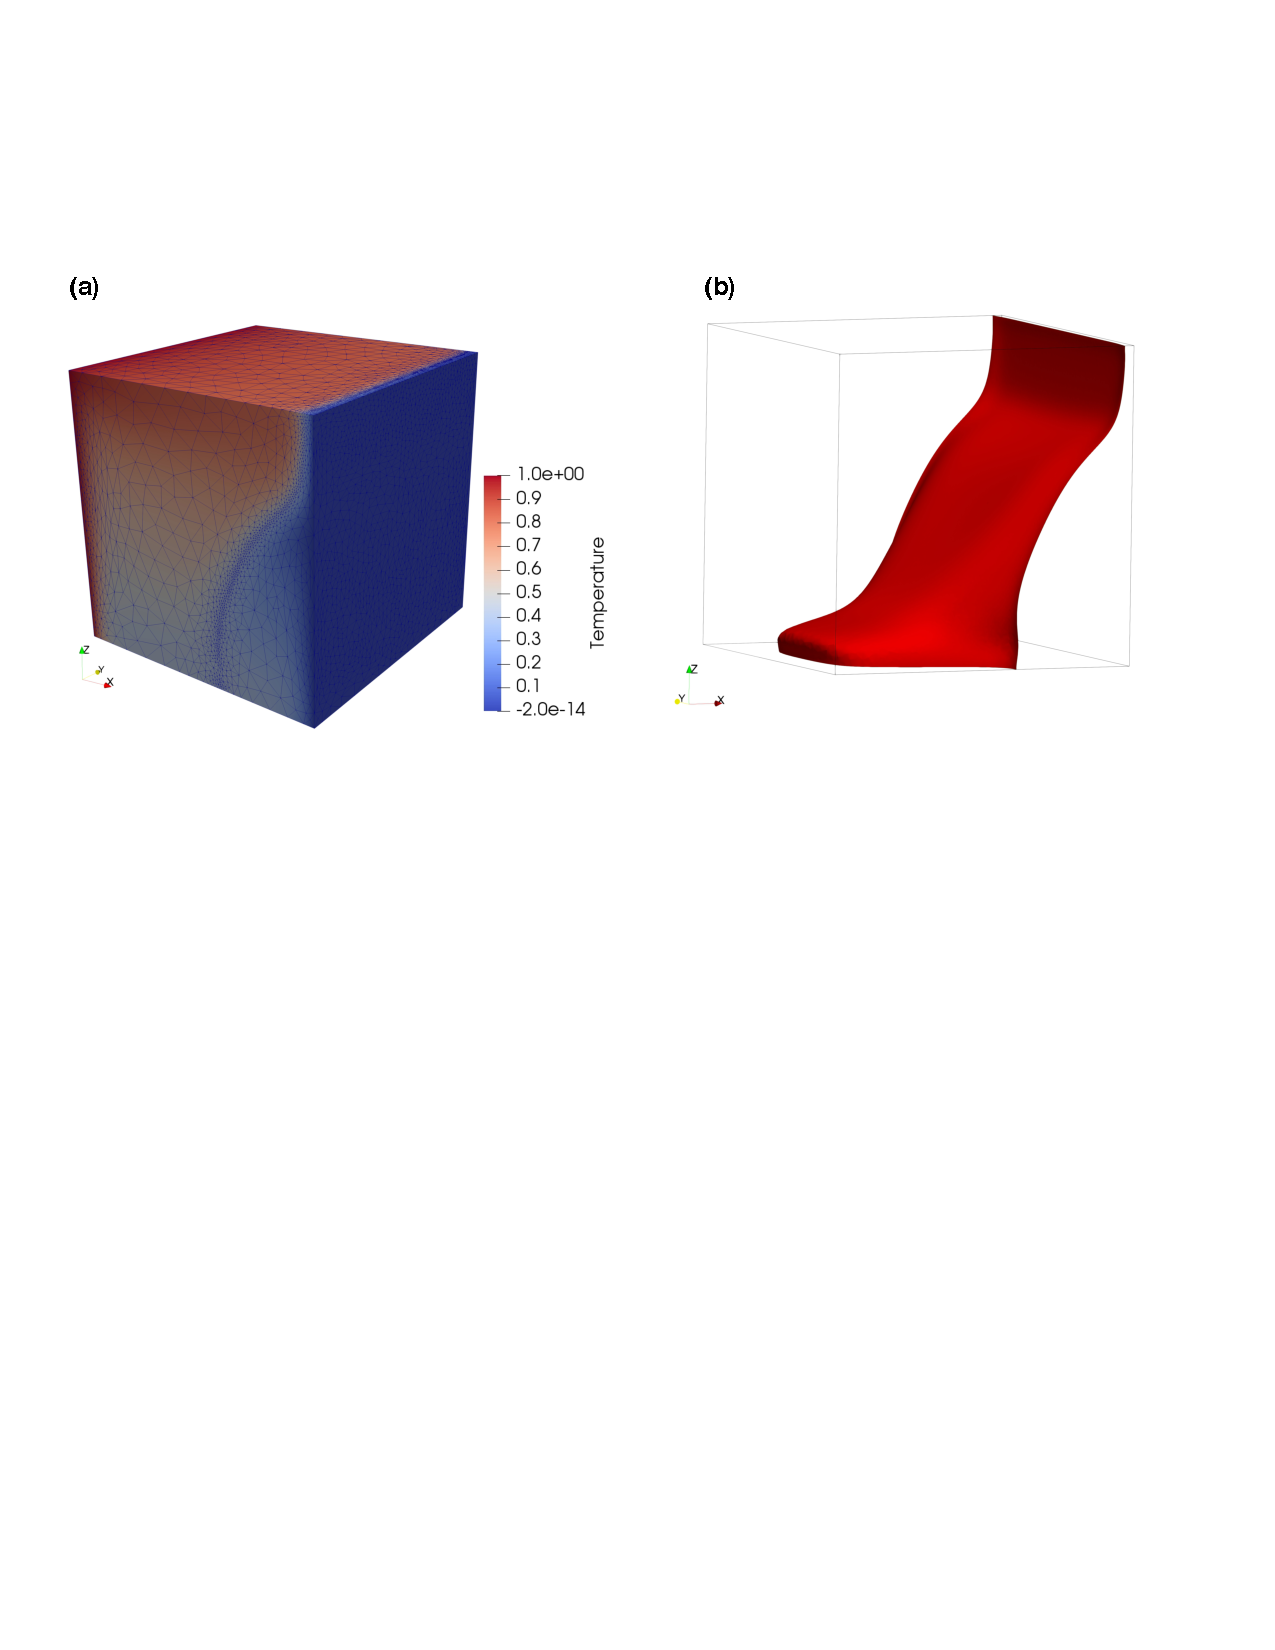
\includegraphics[width=0.9\textwidth]{\figpath/Fig_cap_natconv/3D_WaterConvec}}
 {\includegraphics[width=0.9\textwidth]{\figpath/Fig_cap_natconv/3D_WaterConvec_2}}
\end{minipage}
\end{center}
\caption{Natural convection of water in a cube-shape cavity. (a) Temperature distribution and adapted mesh. (b) Zoom of the 3D adapted mesh at mid-plane. (c) Iso-surface $\theta = \theta_m$. Comparison of the profile of the vertical velocity along $z-$direction with the numerical benchmark by  \cite{Kowalewski-1999} at the mid-plane ($y=0.5$) and $x = 0.93$ (d); $x = 0.1$ (e); $x = 0.5$ (f).}
\label{fig-3D_Water_convec} 
\end{figure}

\section{Numerical simulations of melting PCM with convection in a 3D configuration} \label{sec-3D_melting}
We now proceed to the $3$D simulation of solid-liquid phase-change problems, starting with the melting of a PCM in a cube-shape domain.
The three-dimensionality of the fluid flow can lead to major differences between the two-dimensional solution in some configurations, as the example of the melting of Gallium.
\cite{wittig2012three} showed that the controversial multi-cellular flow occurs only at the beginning of the melting process in two-dimensional simulations.
Three-dimensional simulations exhibit the absence of a multi-vortex structure at any time step.
They explained these differences  by the presence of walls in the third direction which, suppress the flow. Also the occurrence of weak turbulence in the bulk of the melt prevents the formation of the long-living multicellular flow pattern known from 2D simulations.
The three-dimensional geometry allows the fluid movement in all directions and the friction effect provided by no-slip walls in transverse direction influences the flow.
\cite{wittig2012three} have highlighted the existence of a secondary flow in the transverse direction, as shown in Fig.  \ref{fig-3D_PCM_MELTING}, which has its maximal intensity near the side walls.

We expand the $2$D simulations presented in Chapter \ref{chap-MELTING} to $3$D configurations. Solutions obtained by both configurations are compared to assess on the three-dimensional effects that occur during the melting process.
The configuration of the numerical simulation is sketched in Fig. \ref{fig-3D_PCM_MELTING} and the physical parameters of the run are: $\Ray = 3.27 \cdot 10^5$,  $\Prd = 56.2$, and $\Ste = 0.045$.
The PCM is set initially solid throughout the whole domain. 
As the heating progresses, the natural convection intensifies enough to have a pronounced influence on the shape of the interface.
The shape of the phase-change front at $t = 78.7$ is displayed in Fig. \ref{fig-3D_PCM_MELTING}, showing a nonuniform melting front receding from the top to the bottom of the domain.\\

\begin{figure}[!h]
\begin{center}
\begin{minipage}{\linewidth}
 {\includegraphics[width=\textwidth]{\figpath/Fig_cap_melting/Scheme_setup_3D}}
\end{minipage}
\end{center}
\caption{ Melting of a phase-change material. Problem definition, shape of the solid-liquid interface at $t=78.8$, and temperature distribution in the symmetry plane (a). Scheme of $3$D convection flow near the side wall by \cite{wittig2012three} (b).}
\label{fig-3D_PCM_MELTING} 
\end{figure}


Iso-surfaces of the temperature at $t = 78.8$ are offered in panel (a) of Fig. \ref{fig-isosurface_3D_Melting}.
The melting front is influenced by the flow which rises along the hot wall and moves down along the solid-liquid interface, where it is cooled.
The influence of the secondary flow, defined by  \cite{wittig2012three}, is apparent with respect to the curved shape of the interface in the vicinity of the side-walls in the transverse direction.
The adapted mesh at $t = 78.8$, refined along the iso-surface $\theta = 0$, is shown in Fig. \ref{fig-isosurface_3D_Melting}.

\begin{figure}
\begin{center}
\begin{minipage}{\linewidth}
 {\includegraphics[width=0.98\textwidth]{\figpath/Fig_cap_melting/MELTING_3D_v2}}
\end{minipage}
\end{center}
\caption{Melting of a phase-change material. Temperature iso-surfaces (a) and the corresponding adapted mesh (b) at $t = 78.8$.}
\label{fig-isosurface_3D_Melting} 
\end{figure}

The location of the solid-liquid interface at the mid-plane and the time evolution of the Nusselt number for two and three-dimensional configurations are plotted in Fig. \ref{fig-3D_interface_MELTING}.
The position of the interface in panel (a) displays discrepancies between both melting fronts, but the shape remains in good agreement.
These differences are caused by the increase of the velocity in the liquid flow, induced by the three-dimensional effects, as shown by \cite{wittig2012three}, who have compared the volume-averaged velocity $U_{xyz}$, defined as follows:
\begin{equation}
	U_{xyz} = \int_{\Omega} \sqrt{u_1^2 + u_2^2 + u_3^2} \, dV.
\end{equation}
In our simulations, at $t = 78.7$, we obtained $U_{xyz} = 0.548208$ for $3$D simulations and $U_{xy} = 0.519576$ for $2$D.
However, the time evolution of the heat transfer in panel (b) matches well for $2$ and $3$D simulations, with a maximum difference lower than $1 \%$ at the onset of the convection time, and overlap during all the simulation time.
From an engineering point of view, the latter observation means that if only an assessment of the heat transfer during the phase-change process is sought, a $2$D simulation is enough since it could be performed in a realistic computational time.
The $3$D simulation required $2$ days CPU with $200$ processors, while $45$ minutes on a personal computer is enough for the $2$D configuration, for the investigated Rayleigh number.

\begin{figure}
\begin{center}
  {\includegraphics[width=0.98\textwidth]{\figpath/Fig_cap_melting/MELT_Okada_valid_3D}}
\end{center}
\caption{Comparison between $2$D and $3$D solutions. Location of the interface at $t=78.7$ (a) and the Nusselt number at $x=0$ (b).}
\label{fig-3D_interface_MELTING} 
\end{figure}

\section{Numerical simulation of water freezing in a cubic cavity} \label{sec-3D_Water_FREEZING}
In this section, we present a $3$D simulation of the challenging case of ice formation inside differentially heated cubic cavity.
Starting from the steady solution shown in Fig. \ref{fig-3D_Water_convec}, we drop the cold temperature at the right wall from $\theta_c = 0$ to $\theta_c = -1$ under the temperature of fusion (which correspond to physical temperatures $T = 0 \, ^o C$ and $T = -10 \, ^o C$, respectively).
Solid crust arises thus from the cold wall and expands towards the left wall.

The temperature distribution and the adapted mesh at final time $t_{\varphi} = 2340$ s ($t = 1.61$) are displayed in Figs. \ref{fig-3D_Water_Freeze}a and \ref{fig-3D_Water_Freeze}b.
When compared with the natural convection case in Sec. \ref{sec: natconv-air-3D}, the mesh is additionally adapted along the solid moving front, localized by the temperature iso-surface $\theta = 0$.
For the visual identification of the flow structures during the ice formation, panel (c) plots the snapshots of velocity vectors, the iso-surface $\theta = 0.4$ along the anomalous density variation, and the phase-change front at time instant $t = 1.61$.
The effect of the secondary flow, discussed in Sec. \ref{sec-3D_melting}, is also visible by the curved shape of the iso-surface $\theta = \theta_m$ in the transverse $y-$ direction.
One can note however, that the shape of the solidification front is almost $2$D.
The buoyancy-induced fluid motion in the abnormal recirculation region is too weak to influence the solid front. Finally, the overlay of the experimental image of \cite{Kowalewski-1999} and the current simulation exhibits good agreement for the location of the solid-liquid interface.
Differences come mainly from the fact that the undercooling phenomenon during the solidification stage is not taken into account by our model.
However, the global shape of the interface agrees qualitatively with the experimental observation.

\begin{figure}[!ht]
\begin{center}
\begin{minipage}{\linewidth}
 {\includegraphics[width=0.9\textwidth]{\figpath/Fig_cap_melting/Water_Freezing_3D}}
\end{minipage}
\end{center}
\caption{Freezing of pure water in a 3D cubical cavity.  (a) Temperature distribution and adapted mesh at $t_{\varphi}=2340 [s]$. (b) Zoom of the adapted mesh at the mid-plane. (c) Temperature iso-surfaces $\theta=0.4$ and $\theta = 0$ with the velocity vectors in the liquid phase. (d) Superimposition of the interface obtained in the present simulation (red line) on the experimental image of \cite{Kowalewski-1999}.}
\label{fig-3D_Water_Freeze} 
\end{figure}

\section{Concluding remarks}
We developed parallel $3$D tools to simulate natural convection flow involving melting or solidification boundary condition, using domain decomposition method.
The numerical simulations investigated with the recent library \texttt{ffddm} in \ff showed good agreement with the benchmark solutions and the sequential algorithm for all simulated cases.
The qualitative behavior and the topology of the interface for phase-change problems, were discussed in detail.
Three-dimensional effects of the flow were exhibited by the deformed shape of the interface in the transverse direction.
The adaptive $3$D mesh procedure proved very efficient to capture several interfaces, at in the example of the water freezing case.
Grid refinement effort was concentrated only in regions displaying high gradients of the computed variables, and $10$ larger tetrahedra were applied elsewhere.
